\question*{
    Simple Square Pulse Generator
}

The following circuit was used to generate the square waves. The mismatched
values were due to unavailability of matching capacitors. Resistors were
adjusted accordingly. The time period is simply proportional to the capacitors
and resistors connected together.

\begin{equation}
  T = 0.69 RC
\end{equation}

\begin{figure}[ht]
    \centering
    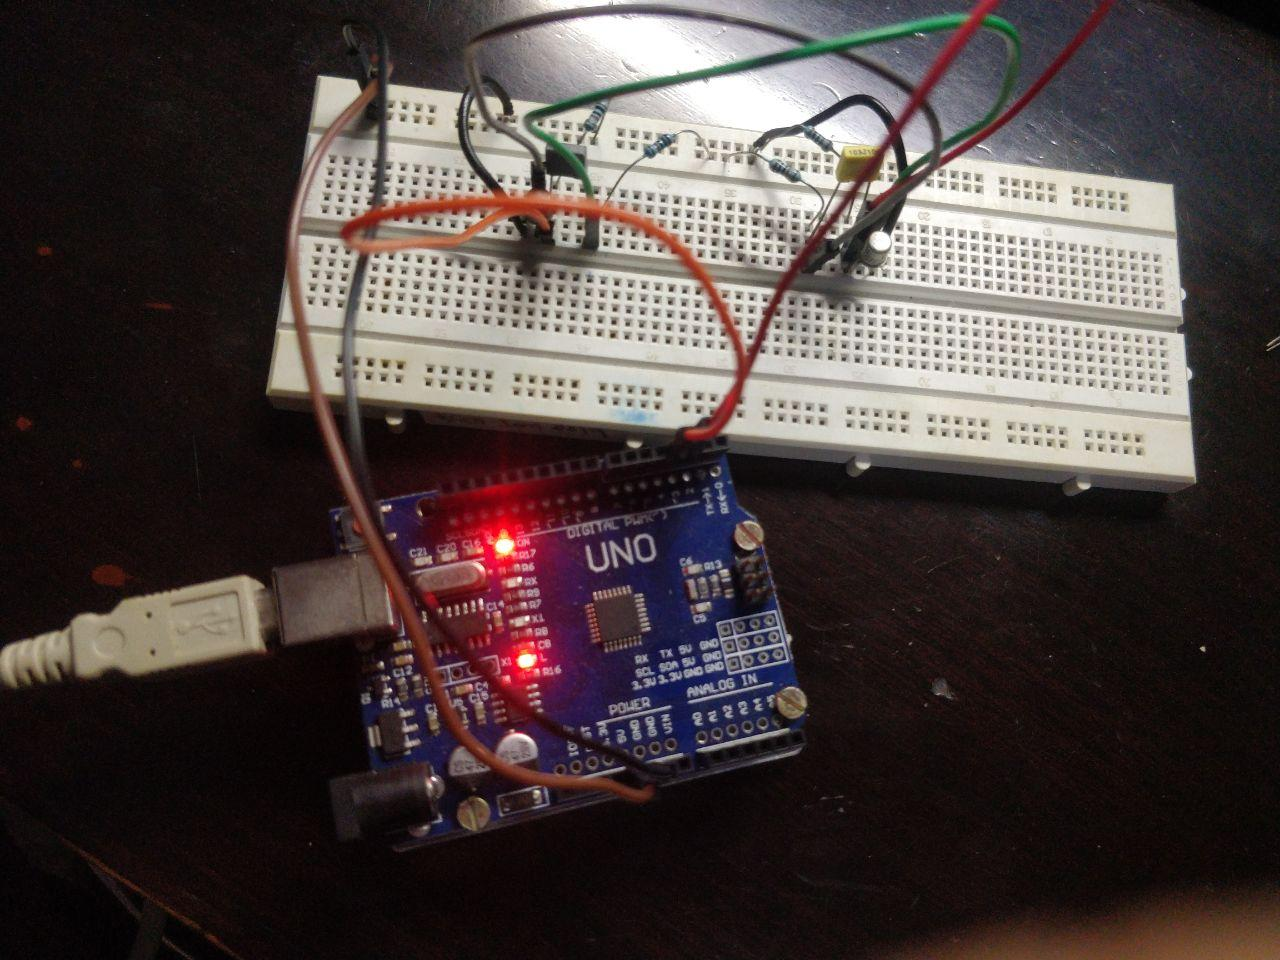
\includegraphics[width=0.6\textwidth]{fig/arduinoconnected-min.jpg}
    \caption{Connected Arduino}
    \label{fig:conn}
\end{figure}

\begin{figure}[ht]
    \centering
    \scalebox{0.5}{\input{fig/circ.pdf_tex}}
    \caption{Oscillator}
    \label{fig:oscillator}
\end{figure}

The circuit simulation is as in \autoref{fig:circsim}

\begin{figure}[ht]
    \centering
    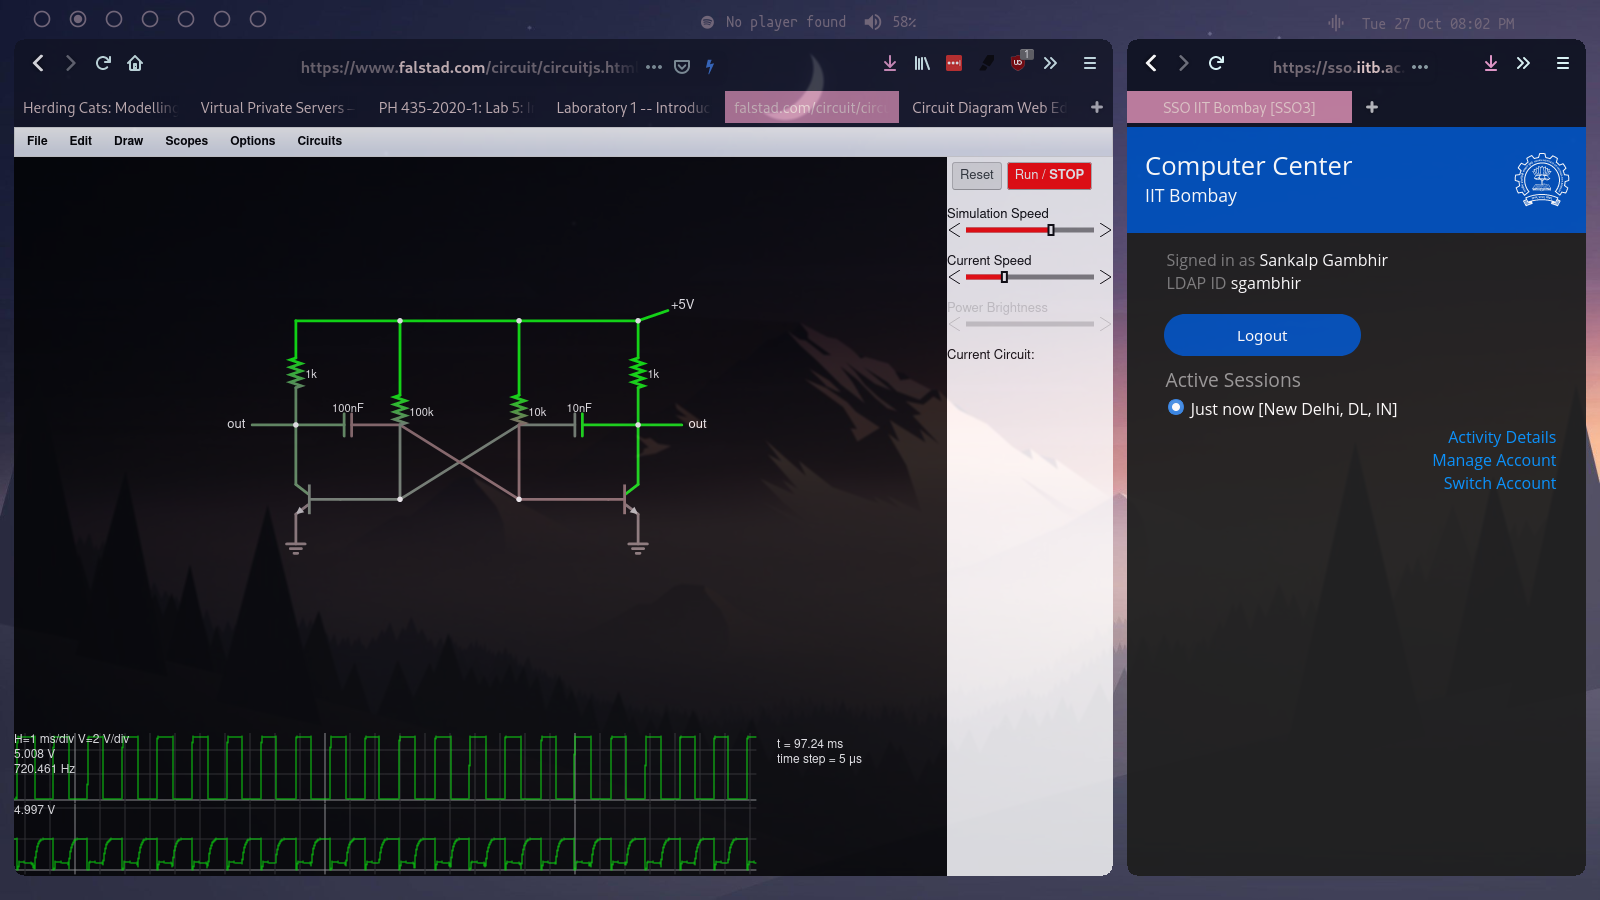
\includegraphics[width=0.8\textwidth]{fig/sim.png}
    \caption{Circuit Simulation}
    \label{fig:circsim}
\end{figure}

\question*{Average speed of a motor}

Code works, see \autoref{fig:sso}. I observed a frequency of about
\textbf{663 Hz}, which is reasonably close to the expected 720Hz from
simulation. 

The state transition diagram is as follows

\begin{figure}[h]
    \centering
    \begin{tikzpicture}
        \node[state]          (q2)  {\texttt{Count}};
        \node[state] at (6,0) (q1)  {\texttt{Report}};

        \draw (q1) edge[bend left, below] node{periodic interrupt}                            (q2)
              (q2) edge[bend left, above] node{\texttt{edgeCount > minEdges}} (q1)
              (q2) edge[loop left]       node{\texttt{edgeCount <= minEdges}}  (q2);
            \end{tikzpicture}
    \caption{State Diagram for Frequency Measuring}
    \label{fig:p2sd}
    \end{figure} 
